\section{CIDR}

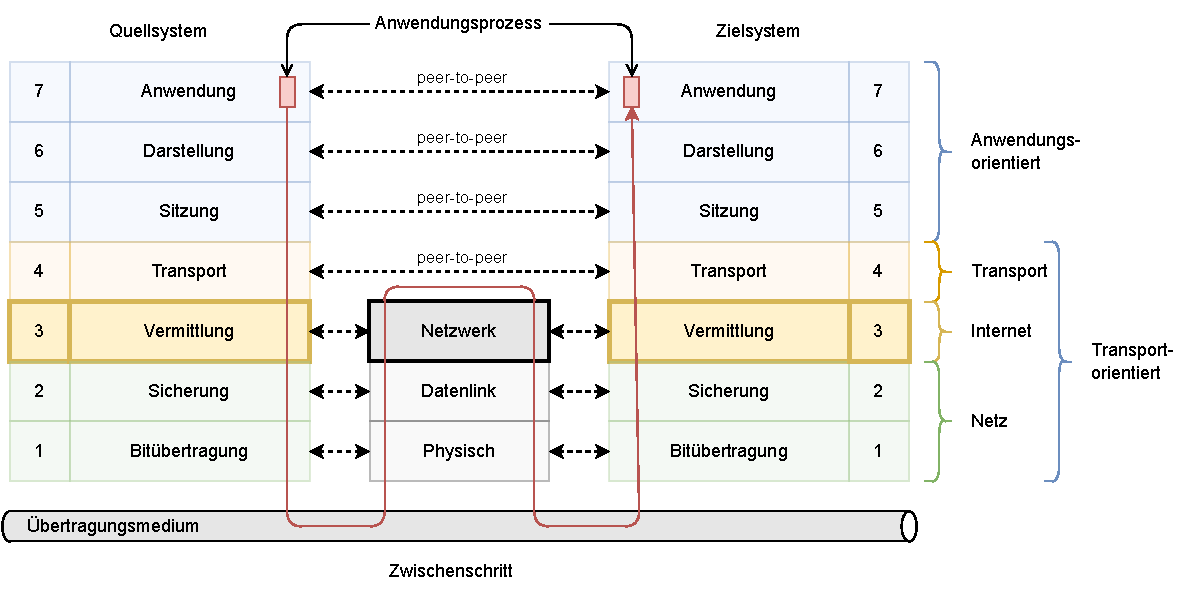
\includegraphics[width=\textwidth]{includes/figures/defi_iso_osi_network.pdf}

\begin{defi}{CIDR}
    \emph{Classless Inter-Domain Routing (CIDR)} beschreibt ein Verfahren zur effizienteren Nutzung des bestehenden 32-Bit-IP-Adress-Raumes für IPv4.

    Mit CIDR entfällt die feste Zuordnung einer IPv4-Adresse zu einer Netzklasse (A, B, C, $\ldots$), aus welcher aus den ersten beiden Bits des ersten Oktetts die Präfixlänge der jeweiligen Netzklasse hervorging.

    Die Präfixlänge ist mit CIDR frei wählbar und muss deshalb beim Aufschreiben eines IP-Subnetzes mit angegeben werden.
    Dazu verwendet man häufig eine \emph{Netzmaske}.

    Bei CIDR führte man als neue Notation so genannte Suffixe ein.
    Das Suffix gibt die Anzahl der 1-Bits in der Netzmaske an.\footnote{Bei IPv6 ist die Notation gleich wie beim CIDR in IPv4 und besteht aus IPv6-Adresse und Präfixlänge.}
\end{defi}

\begin{bonus}{Probleme IPv4}
    Da nur ca. 4.3 Mrd. ($2^{32}$) Adressen zur Verfügung stehen, kann nicht jedes Gerät eine eigene weltweit eindeutige IP-Adresse erhalten.
    Anfänglich hatte niemand damit gerechnet, dass dieses neue Phänomen \enquote{Internet} derart stark wächst.

    Um dieses Problem zu lösen, bzw. die resultierenden Auswirkungen aufzuschieben, wurden private Netze eingeführt.
    Da ebenfalls festgestellt wurde, dass Adressklassen auf Grund hoher Verschwendung an überschüssigen IP Adressen nicht zielführend war\footnote{
        Wenn man mehr als 254 Endgeräte anschließen möchte, benötigt man bereits ein Klasse B Netz.
        Es bleiben bis zu 64.281 Adressen ungenutzt
    }, konnte man die Grenze zwischen Netz-ID und Knoten-ID nun beliebig wählen.
    Alternativ erhält man mehrere kleine Netze, die man durch Router verbinden muss.

    Jedes IP Netz benötigt ab jetzt ebenfalls eine Subnetzmaske.
    Diese wird genutzt um eindeutig zwischen Netz und Knoten-ID zu unterscheiden.

    Die Subnetzmaske kann entweder in IPv4- oder in CIDR-Schreibweise angegeben werden.
    In CIDR wird die Anzahl der 1en in der Subnetzmaske hinter der IPv4 Adresse angegeben. Die Stellen der Knoten-ID können weggelassen werden.

    Um eine gewisse Struktur in private Netze zu bringen, wurden gewisse Richtlinien geschaffen, um aus den historischen Klassen private Netze zu erstellen.
    Jedes übersetzte Netz hat 24 frei wählbare Stellen.
    Im Gegensatz dazu kann man in eigenen privaten Netzen alle Stellen der IP-Adresse frei wählen.
    Dabei entscheidet die Länge der Subnetzmaske ($\text{snm}$) über die Anzahl der verfügbaren IPv4-Adressen ($2^{32-\text{snm}}$).
    \begin{center}
        \begin{tabular}{|c|l|l|l|l|}
            \hline
            Klasse & CIDR-Notation         & Anzahl Netze & Anzahl Adressen         & Netze                     \\\hline\hline
            A      & \texttt{10/8}         & $2^0 = 1$    & $2^{24} = 16.777.216$   & \texttt{10/8}             \\\hline
            B      & \texttt{172.16/12}    & $2^4 = 16$   & $2^{20} = 1.048.576$    & \texttt{172.16/16} bis    \\
                   &                       &              &                         & \texttt{172.31/16}        \\\hline
            C      & \texttt{192.168/16}   & $2^8 = 256$  & $2^{16} = 65.536$       & \texttt{192.168.0/24} bis \\
                   &                       &              &                         & \texttt{192.168.255/24}   \\\hline
            /24    & \texttt{192.168.0/24} &              & $2^{32-24} = 2^8 = 256$ &                           \\\hline
        \end{tabular}
    \end{center}
\end{bonus}

\begin{example}{IPv4-Netz}
    Betrachten wir ein typisches IPv4-Netz mit Subnetzmaske:
    \texttt{192.168.0.0} mit \texttt{255.255.255.0}

    bzw. in CIDR:
    \texttt{192.168.0.0/24} bzw. \texttt{192.168.0/24}

    Wenn wir eine beliebige IP-Adresse aus diesem Netz erhalten, können wir mithilfe logischer Gatter zuerst das Netz eindeutig identifizieren, und dann den Host adressieren.

    z.B. \texttt{192.168.0.4/24}

    \begin{center}
        \begin{tabular}{|l||c|l|}
            \hline
            IP-Adresse                                                                                     & \texttt{1100 0000 . 1010 1000 . 0000 0000 . 0000 0100}          & \texttt{192.168.0.4}          \\\hline
            Subnetzmaske                                                                                   & \texttt{1111 1111 . 1111 1111 . 1111 1111 . 0000 0000}          & \texttt{255.255.255.0}        \\\hline
            Netz-ID\footnote{$\text{Netz-ID} = \text{IP-Adresse} \land \text{Subnetzmaske}$}               & \texttt{\textbf{1100 0000 . 1010 1000 . 0000 0000} . 0000 0000} & \texttt{\textbf{192.168.0}.0} \\\hline
            Geräte-ID\footnote{$\text{Geräte-ID} = \text{IP-Adresse} \land	\overline{\text{Subnetzmaske}}$} & \texttt{0000 0000 . 0000 0000 . 0000 0000 . \textbf{0000 0100}} & \texttt{0.0.0.\textbf{4}}     \\\hline
        \end{tabular}
    \end{center}
\end{example}

\begin{example}{IP-Subnetze}
    Nehmen wir das Klasse B Netz der RWTH Aachen University:
    \texttt{134.130.0.0}\footnote{
        Netz-Adresse startet in binär mit \texttt{10}.
        Daher wissen wir, dass es sich um ein Klasse B Netz handelt
    }

    In diesem Klasse B Netz sind folgende Subnetze gegeben:\\
    \texttt{134.130.1.0/24}\\
    \texttt{134.130.2.0/24}\\
    \texttt{134.130.3.0/24}

    Durch die Subnetzmaske wissen wir, dass die Netz-ID die ein Byte länger ist, als die Netz-ID der Netzklasse (Klasse B hat \texttt{/16}).
    Dementsprechend können wir bis zu $2^8 = 256$ Subnetze mit jeweils bis zu 254\footnote{
        Obacht: Die logische Aufteilung in Subnetze ist sinnvoll, jedoch gehen bei jedem Subnetz jeweils zwei IP-Adressen für Netz-Adresse und Broadcast verloren.
        Dementsprechend sollte man Subnetze ausschließlich für unabhängige Instanzen nutzen.
        z.B. Institute der RWTH, Dezernate der FH-Aachen etc.
    } Endgeräten erstellen.

    z.B. \texttt{134.130.1.4/24}

    \begin{center}
        \begin{tabular}{|l||c|l|}
            \hline
            IP-Adresse                                                                                                                     & \texttt{1000 0110 . 1000 0010 . 0000 0001 . 0000 0100}          & \texttt{134.130.1.4}          \\\hline
            Subnetzmaske                                                                                                                   & \texttt{1111 1111 . 1111 1111 . 1111 1111 . 0000 0000}          & \texttt{255.255.255.0}        \\\hline
            IP-Klassenmaske\footnote{Bekannt durch IP-Klassenpräfix}                                                                       & \texttt{1111 1111 . 1111 1111 . 0000 0000 . 0000 0000}          & \texttt{255.255.0.0}          \\\hline
            Netz-ID\footnote{$\text{Netz-ID} = \text{IP-Adresse} \land \text{Subnetzmaske} \land \text{IP-Klassenmaske}$}                  & \texttt{\textbf{1000 0110 . 1000 0010} . 0000 0000 . 0000 0000} & \texttt{\textbf{134.130}.0.0} \\\hline
            Subnetz-ID\footnote{$\text{Subnetz-ID} = \text{IP-Adresse} \land \text{Subnetzmaske} \land \overline{\text{IP-Klassenmaske}}$} & \texttt{0000 0000 . 0000 0000 . \textbf{0000 0001} . 0000 0000} & \texttt{0.0.\textbf{1}.0}     \\\hline
            Geräte-ID\footnote{$\text{Geräte-ID} = \text{IP-Adresse} \land	\overline{\text{Subnetzmaske}}$}                                 & \texttt{0000 0000 . 0000 0000 . 0000 0000 . \textbf{0000 0100}} & \texttt{0.0.0.\textbf{4}}     \\\hline
        \end{tabular}
    \end{center}
\end{example}

\begin{defi}{Longest Prefix Match}
    Beim \emph{Longest Prefix Match} geht es darum, wie ein Router möglichst effizient eine maximal mögliche Übereinstimmung der Zieladresse mit einer gespeicherten IP-Adresse aus seiner internen Routingtabelle findet.

    Der Routenalgorithmus kommt dann zum Einsatz, wenn die Routingtabelle mehrere potentiell zur Zieladresse eines Paketes passende Adressbereiche beinhaltet, und gehört nach der Ablösung Netzklassen durch Adressen und frei wählbare Netzmasken (CIDR) zu den Standardverfahren.
\end{defi}

\begin{example}{Longest Prefix Match}
    IPv4 Routingtabelle eines Routers:

    \begin{tabular}{|l|l|l|l|}
        \hline
        Nr. & Netzwerk-Adresse        & Subnetzmaske                           & Ziel            \\
        \hline \hline
        1   & \texttt{198.51.100.0}   & \texttt{/24}, \texttt{255.255.255.0}   & Schnittstelle 1 \\
        \hline
        2   & \texttt{198.51.100.64}  & \texttt{/26}, \texttt{255.255.255.192} & Schnittstelle 2 \\
        \hline
        3   & \texttt{198.51.100.128} & \texttt{/26}, \texttt{255.255.255.192} & Schnittstelle 3 \\
        \hline
    \end{tabular}

    Es wird ein Paket mit der IPv4-Adresse \texttt{198.51.100.78} empfangen.

    Dann gilt:

    \begin{tabular}{|l|l|l|}
        \hline
        Adresse/Netz (CIDR)        & Binärdarstellung                                                 & Match  \\
        \hline\hline
        \texttt{198.51.100.78/32}  & \texttt{11000110 . 00110011 . 01100100 . 01001110}               &        \\
        \hline\hline
        \texttt{198.51.100.0/24}   & \texttt{\textbf{11000110 . 00110011 . 01100100 . 0}\st{0}000000} & 25 Bit \\
        \hline
        \texttt{198.51.100.64/26}  & \texttt{\textbf{11000110 . 00110011 . 01100100 . 01}000000}      & 26 Bit \\
        \hline
        \texttt{198.51.100.128/26} & \texttt{\textbf{11000110 . 00110011 . 01100100} . \st{10}000000} & -      \\
        \hline
    \end{tabular}

    Die längste Übereinstimmung mit dem jeweiligen vollständigen fixen Adressteil liegt bei Eintrag 2 vor, nämlich 26 Bit.

    Weiterleitung des Paketes entsprechend über Schnittstelle 2.
\end{example}

\begin{bonus}{Verkleinerung der Routing-Tabelle durch CIDR}
    Der Longest Prefix Match erlaubt das Zusammenfassen von Routen.

    Zu beachten ist:
    \begin{itemize}
        \item Ein Zusammenfassen ist nur möglich, wenn gleiche Ziele verwendet werden.
        \item Die relaxierte interpretation der Netzwerkadresse kann ggf. andere, nicht gewollte Einträge umfassen.\footnote{Hier hilft ggf. die Longest Prefix Match-Regel. Hierzu muss aber der Präfix der überschriebenen Regel länger sein.}
        \item \texttt{0.0.0.0/0} ist die Default-Route.
    \end{itemize}
\end{bonus}